\documentclass[12pt,a4paper]{report}
\usepackage[margin=2.50cm]{geometry}
\usepackage{subcaption,graphicx}
%\usepackage[section]{placeins}

\title{Implementing a Univariate Gaussian Classifier}

\begin{document}
\maketitle
\section{What is classification?}

\section{Steps}
\begin{enumerate}
	\item Train
	\item Perform classification
	\item Test and estimate error
\end{enumerate}

\section{Training}
\subsection{What is a mask?}
\begin{figure}
\centering
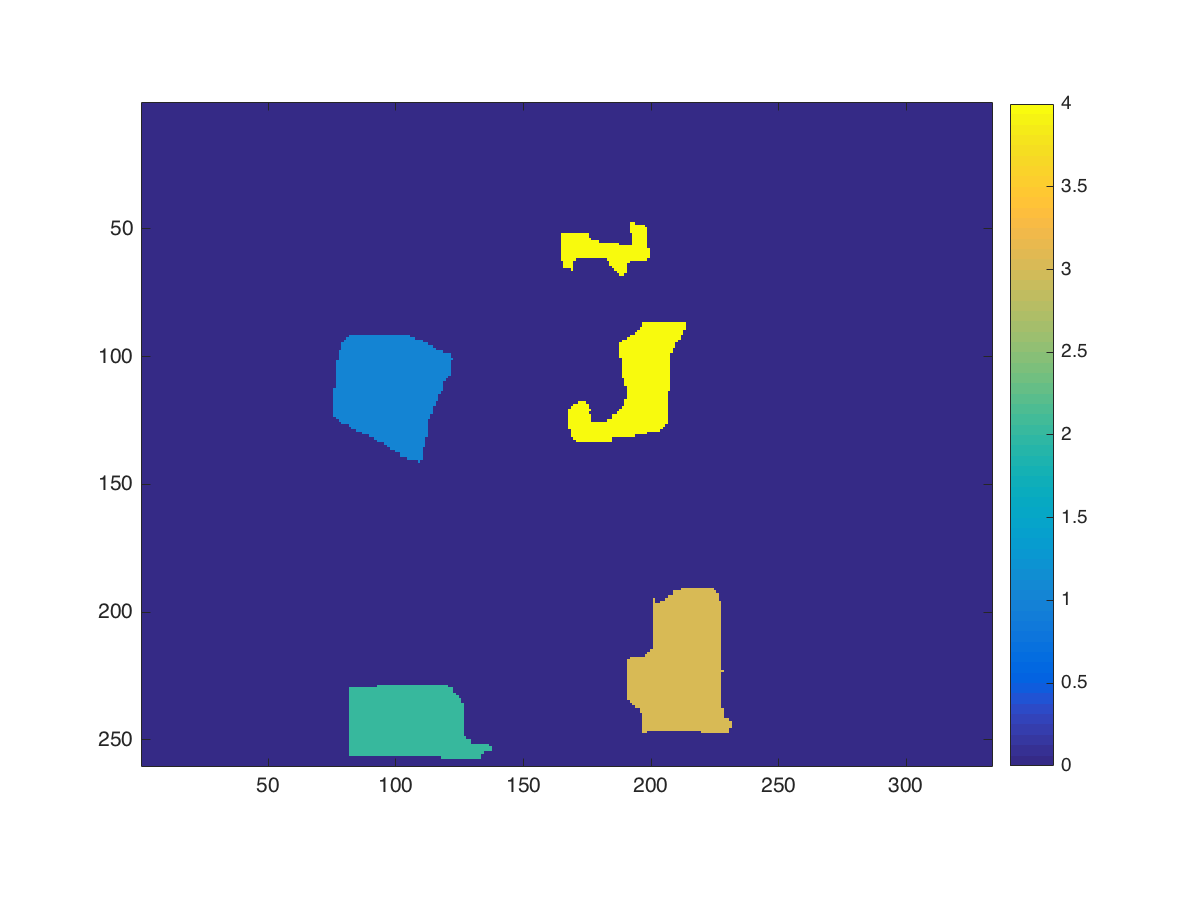
\includegraphics[width=0.75\textwidth]{TrainingMask}
\caption{A training mask}
\label{fig:TrainingMask}
\end{figure}

A mask is used to to train the classifier by identifying known regions as belonging to a particular class. In figure\ref{fig:TrainingMask} we can see a typical mask using 4 arbitrary colors plus the background. Each region of color represents a region known to belong to a class. The numeric value that is being visualized as a color is actually just a label. The background of the image, the dark blue sea, is not part of the training data. It is important to remember, the  choice of dark blue (0) and the other colors (1-4) are an artifact of Matlab's imagesc function and have no special meaning.

\subsection{How do we train using a mask?}
We are now going to roll through an image and train the classifier.
\begin{figure}[!ht]
	\begin{subfigure}{0.5\textwidth}
	\centering
	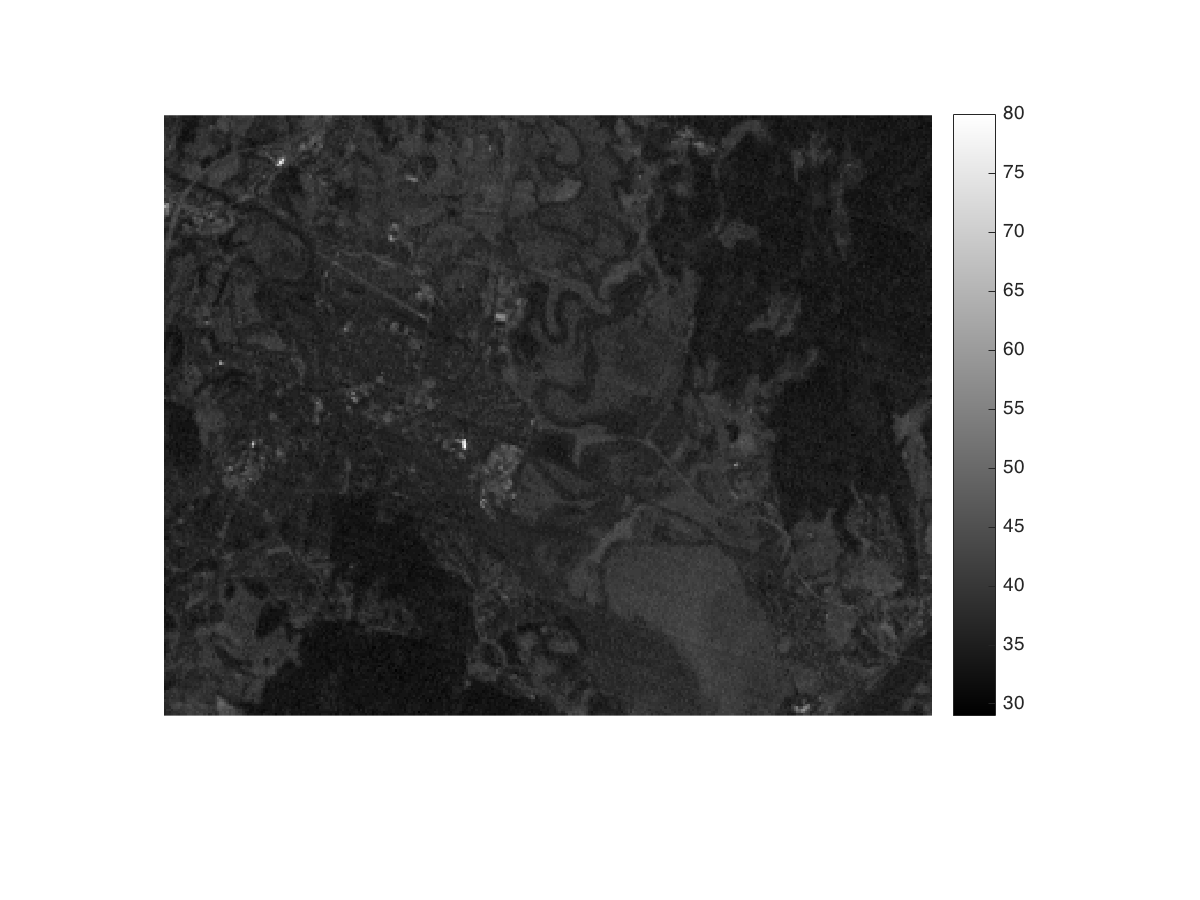
\includegraphics[width=1.0\textwidth]{Landsat1}	
	\caption*{Image 1}
	\end{subfigure}
	\begin{subfigure}{0.5\textwidth}
	\centering
	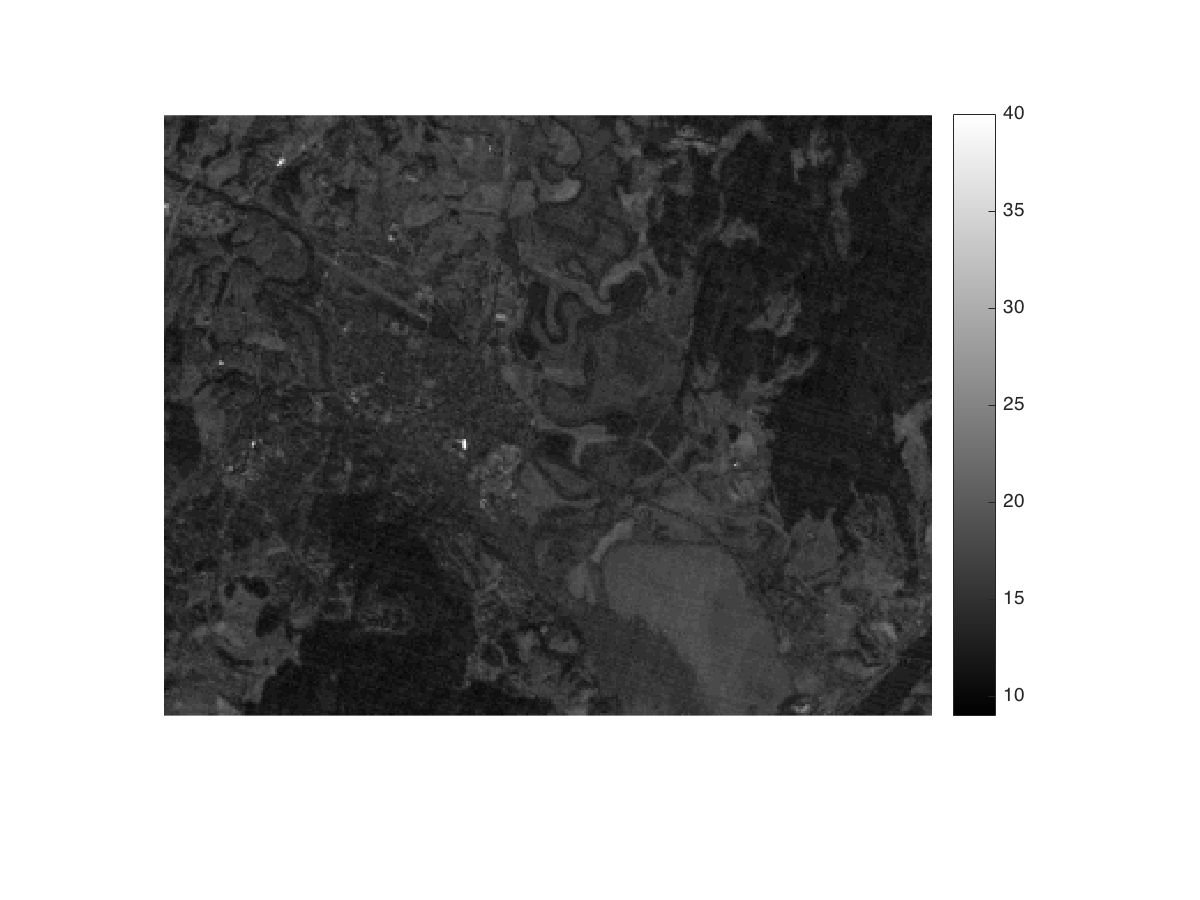
\includegraphics[width=1.0\textwidth]{Landsat2}
	\caption*{Image 2}
	\end{subfigure}
\end{figure}
\begin{figure}[!ht]
	\begin{subfigure}{0.5\textwidth}
	\centering
	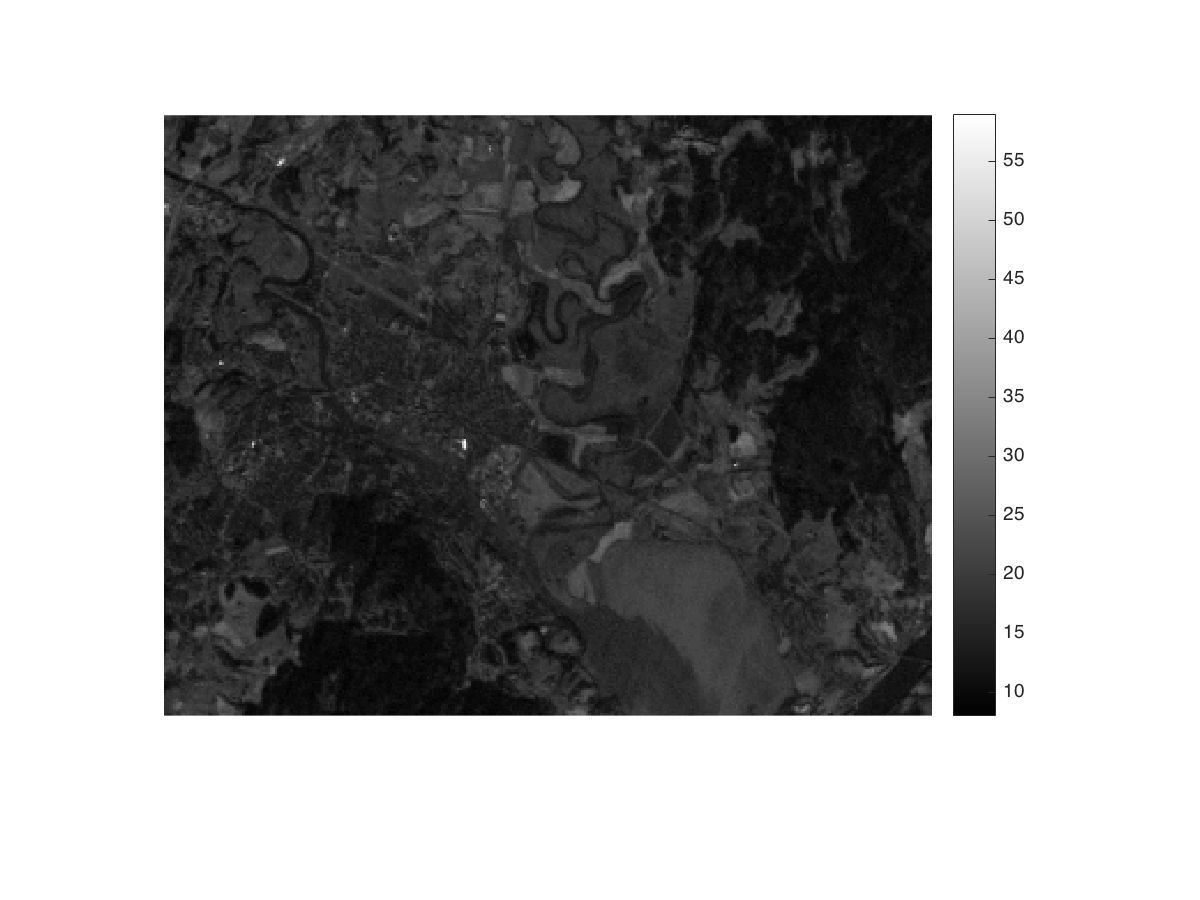
\includegraphics[width=1.0\textwidth]{Landsat3}	
	\caption*{Image 3}
	\end{subfigure} 
	\begin{subfigure}{0.5\textwidth}
	\centering
	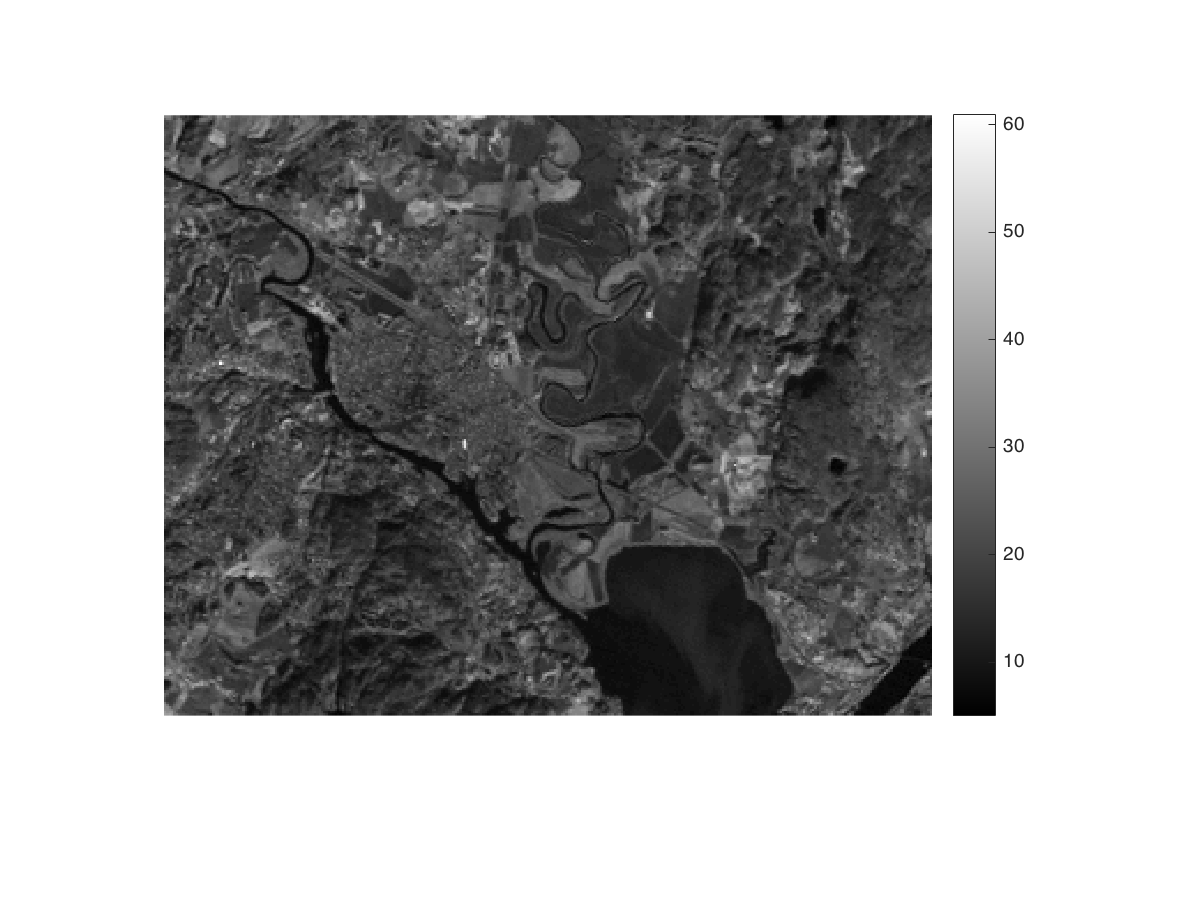
\includegraphics[width=1.0\textwidth]{Landsat4}	
	\caption*{Image 4}
	\end{subfigure}
\end{figure}
\begin{figure}[!ht]
	\begin{subfigure}{0.5\textwidth}
	\centering
	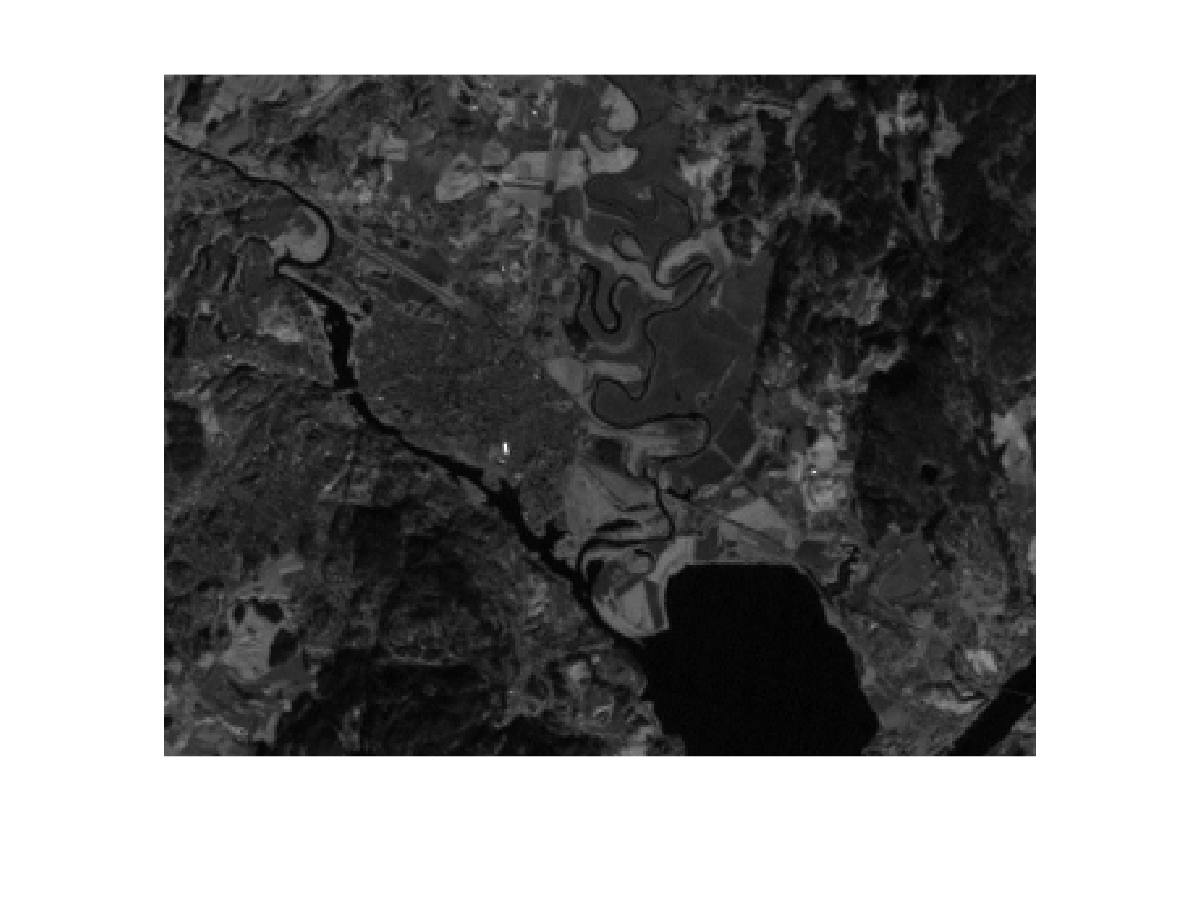
\includegraphics[width=1.0\textwidth]{Landsat5}	
	\caption*{Image 5}
	\end{subfigure}
	\begin{subfigure}{0.5\textwidth}
	\centering
	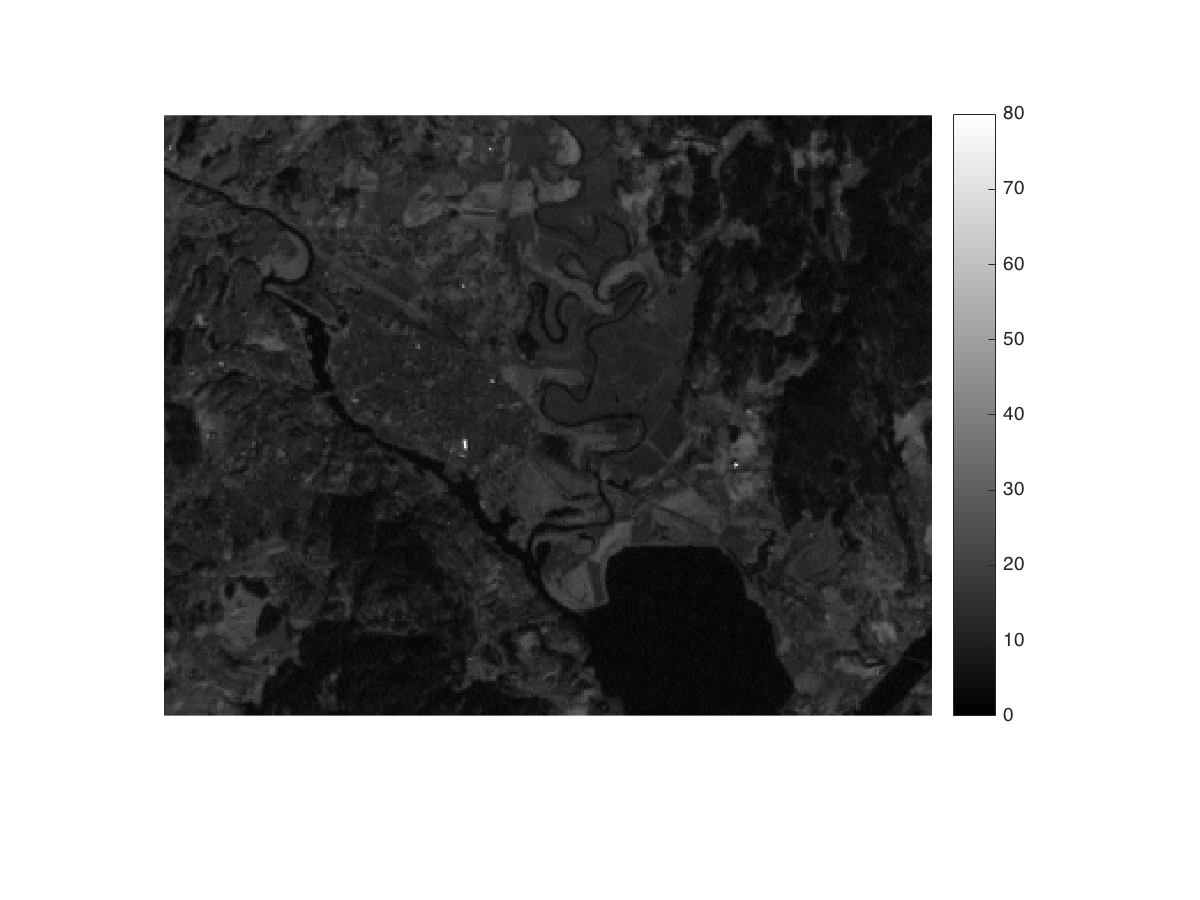
\includegraphics[width=1.0\textwidth]{Landsat6}	
	\caption*{Image 6}
	\end{subfigure}
	\caption{Landsat images at different wavelengths}
\end{figure}

For an image we are interested in, we apply the training mask and  'learn' how to classify all pixels. Practically speaking, for each image we calculate the $\mu$ (mean) and $\sigma^2$ (variance) for each class. So if we imagine a small circle in the middle of an image as being our training mask for class 1 pixels we would average those pixels and then take the variance of those pixels. We would do this for each class in the mask, which in our example included 1-4, so we end up with 4 pairs of mean and variance.

If you're unsure of how to calculate variance check out Wikipedia's article on Standard Deviation, it is refreshingly simple.

\section{Probability Density Function}
To use a classifier we need to select a probability density function. The most commonly used probability density function for the purpose of classification is the normal (Gaussian) distribution. We already have $\mu$ and $\sigma^2$ so the remaining value is $x$ which is the gray level of the pixel.
\begin{equation}
	P(x) = \frac{1}{\sigma\sqrt{2\pi}}e^{-\frac{(x - \mu)^2}{2\sigma^2}}
\end{equation}

Visualizing the probability distributions for each of the 4 classes computed on each of the 6 images gives us some intuition into how well the classifier will perform.

\begin{figure}[!ht]
	\begin{subfigure}{0.5\textwidth}
	\centering
	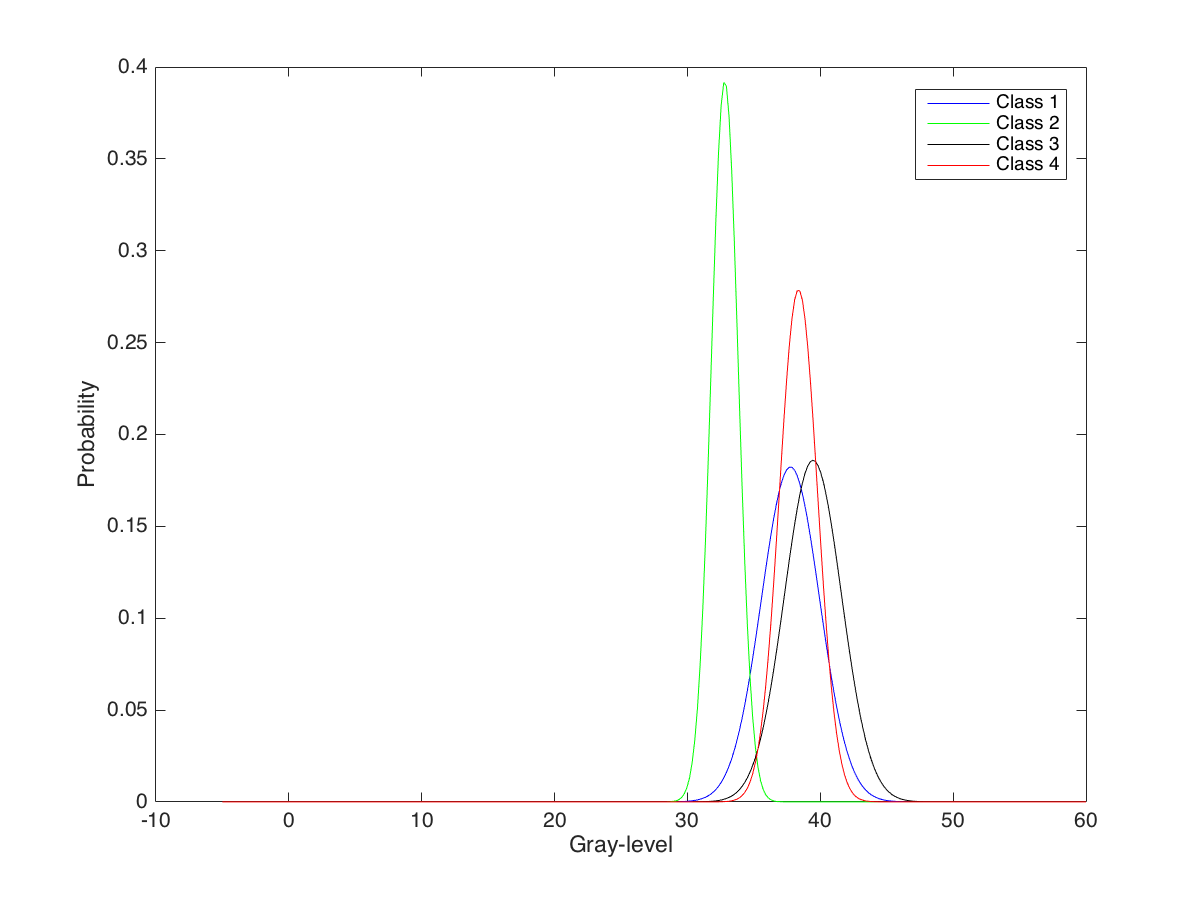
\includegraphics[width=1.0\textwidth]{Feature1ProbabilityDistribution}	
	\caption*{Image 1}
	\end{subfigure}
	\begin{subfigure}{0.5\textwidth}
	\centering
	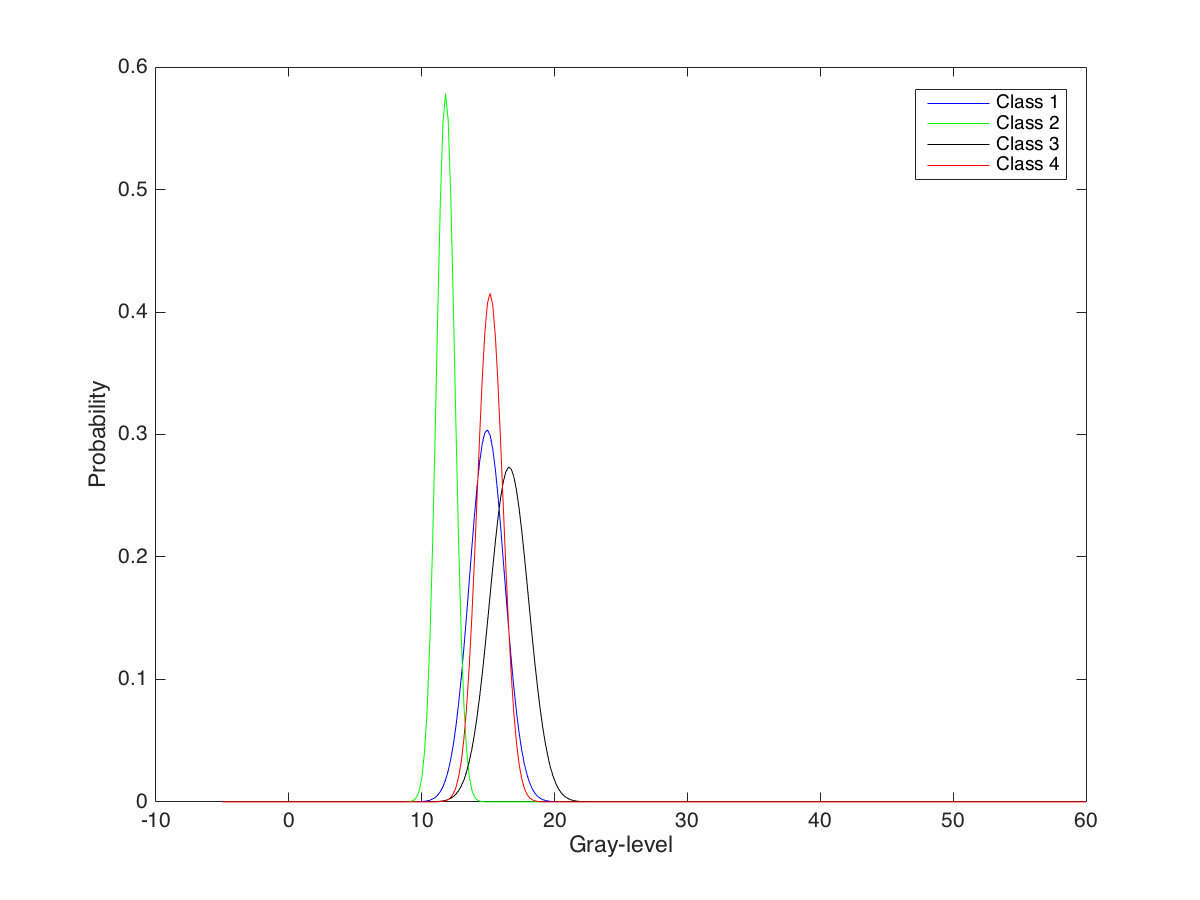
\includegraphics[width=1.0\textwidth]{Feature2ProbabilityDistribution}
	\caption*{Image 2}
	\end{subfigure}
\end{figure}
\begin{figure}[!ht]
	\begin{subfigure}{0.5\textwidth}
	\centering
	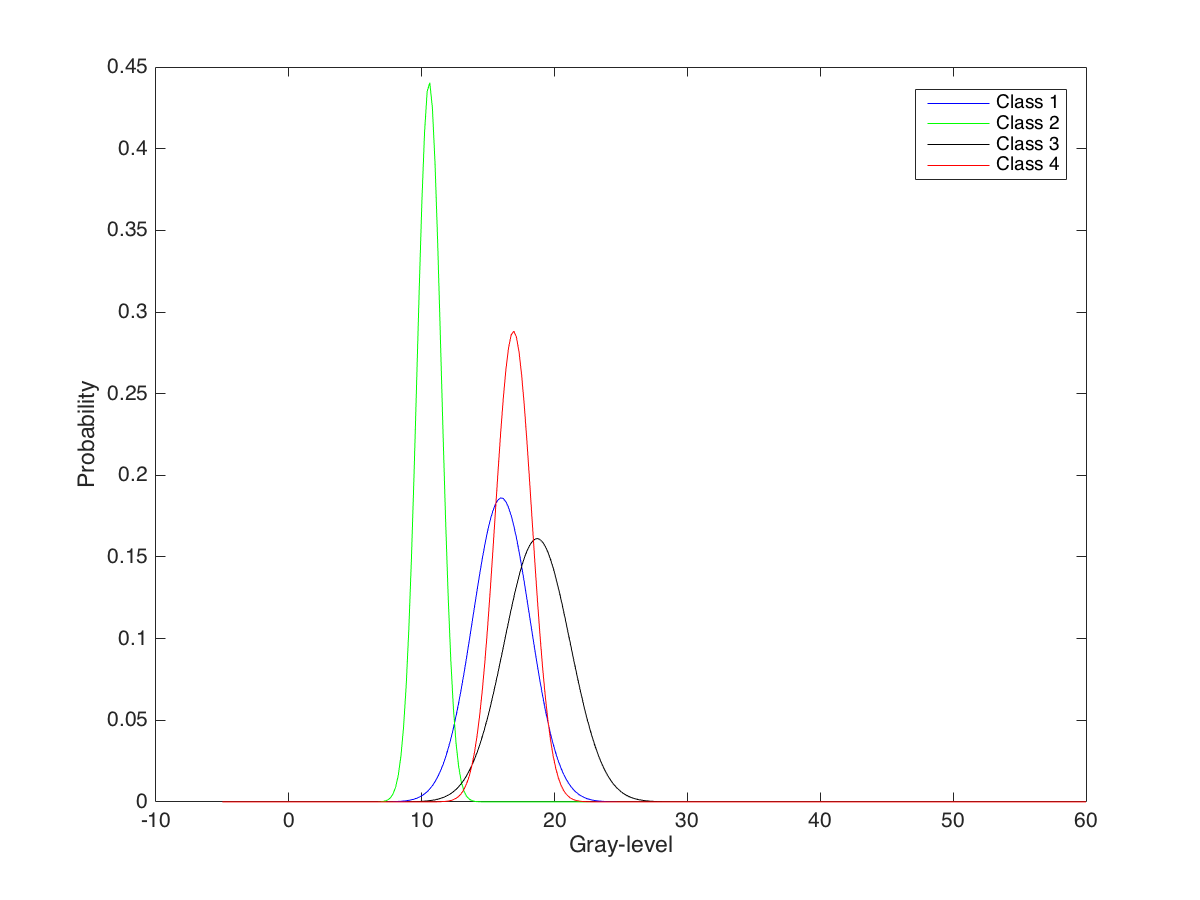
\includegraphics[width=1.0\textwidth]{Feature3ProbabilityDistribution}	
	\caption*{Image 3}
	\end{subfigure} 
	\begin{subfigure}{0.5\textwidth}
	\centering
	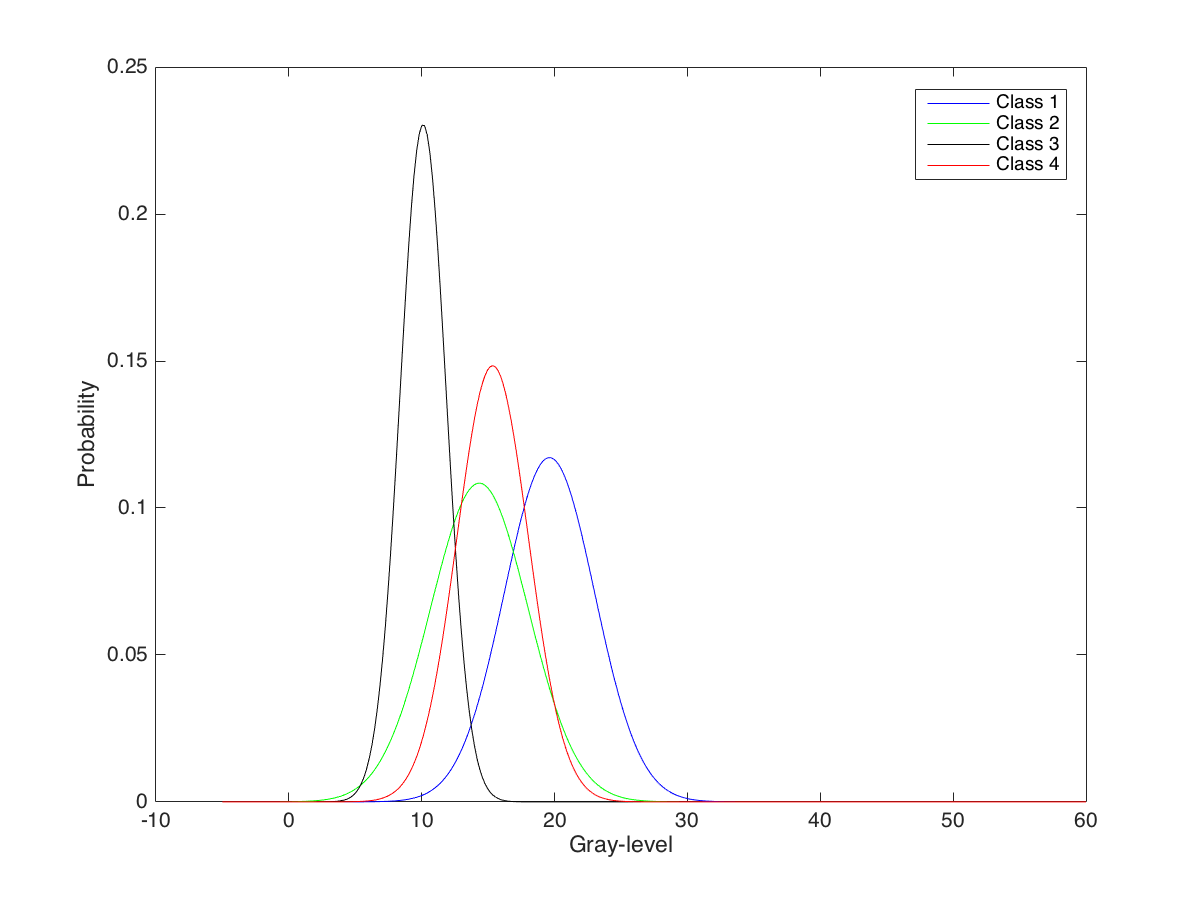
\includegraphics[width=1.0\textwidth]{Feature4ProbabilityDistribution}	
	\caption*{Image 4}
	\end{subfigure}
\end{figure}
\begin{figure}[!ht]
	\begin{subfigure}{0.5\textwidth}
	\centering
	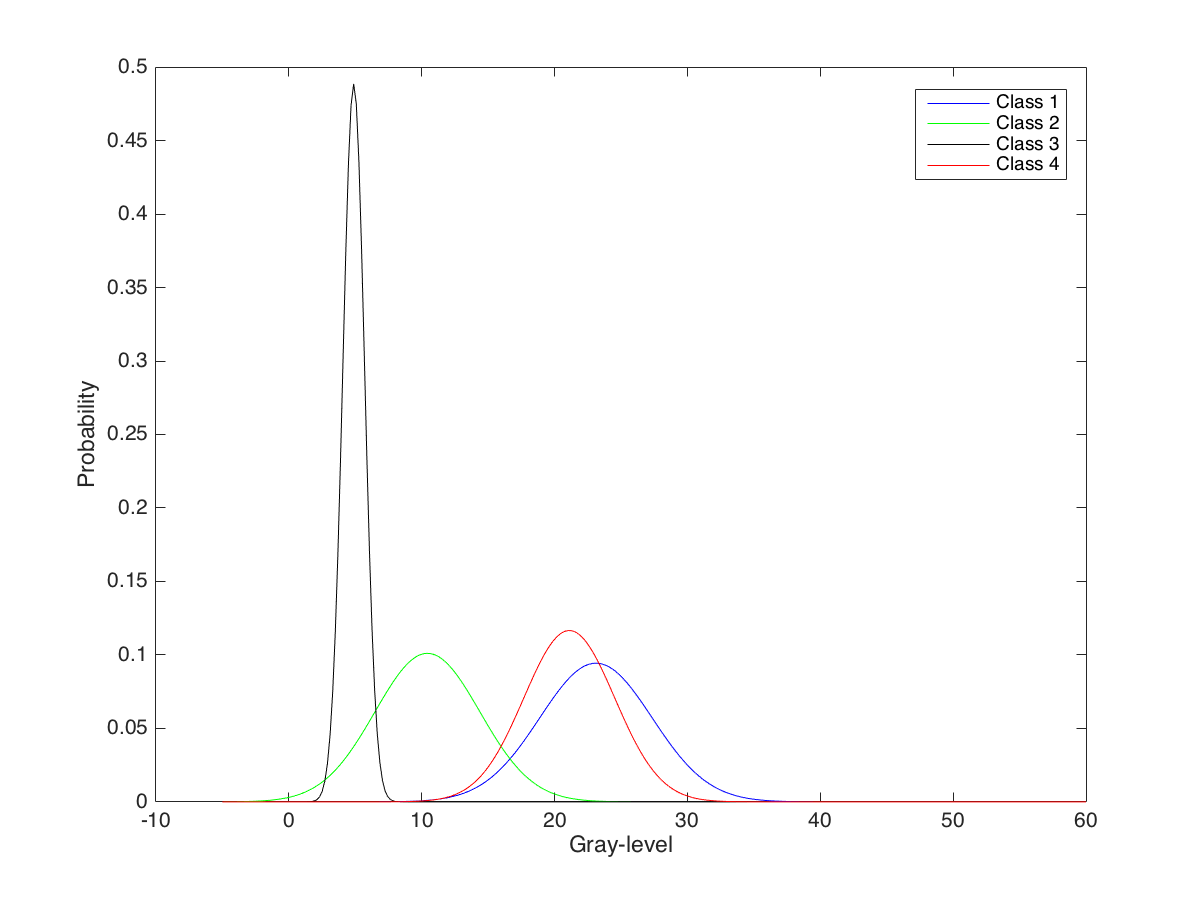
\includegraphics[width=1.0\textwidth]{Feature5ProbabilityDistribution}	
	\caption*{Image 5}
	\end{subfigure}
	\begin{subfigure}{0.5\textwidth}
	\centering
	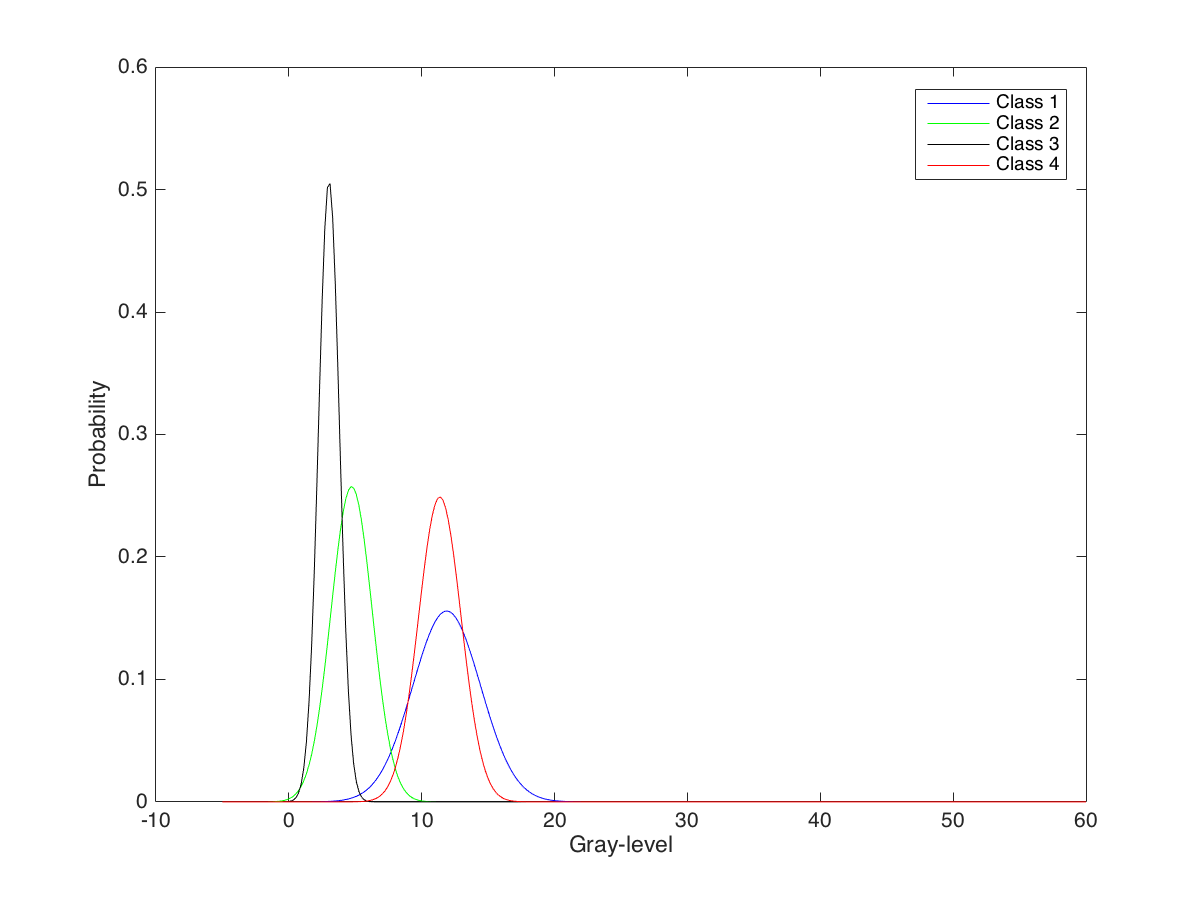
\includegraphics[width=1.0\textwidth]{Feature6ProbabilityDistribution}	
	\caption*{Image 6}
	\end{subfigure}
	\caption{Probability distributions for each image}
\end{figure}

\section*{A now for a brief foray into how the Probability Density function is derived, or what is Bayes Theorem and how can it be applied using a normal distribution?}

Explain Bayes Theorem and the Gaussian distribution here.

\section*{Classifying}
So using our probability density function we roll through all the pixels in the image testing the gray level, with each pair of mean and variance. In our case, 4 calculations per pixel. Whichever class yields the highest probability wins. Record the  result.

\begin{figure}[!ht]
	\begin{subfigure}{0.5\textwidth}
	\centering
	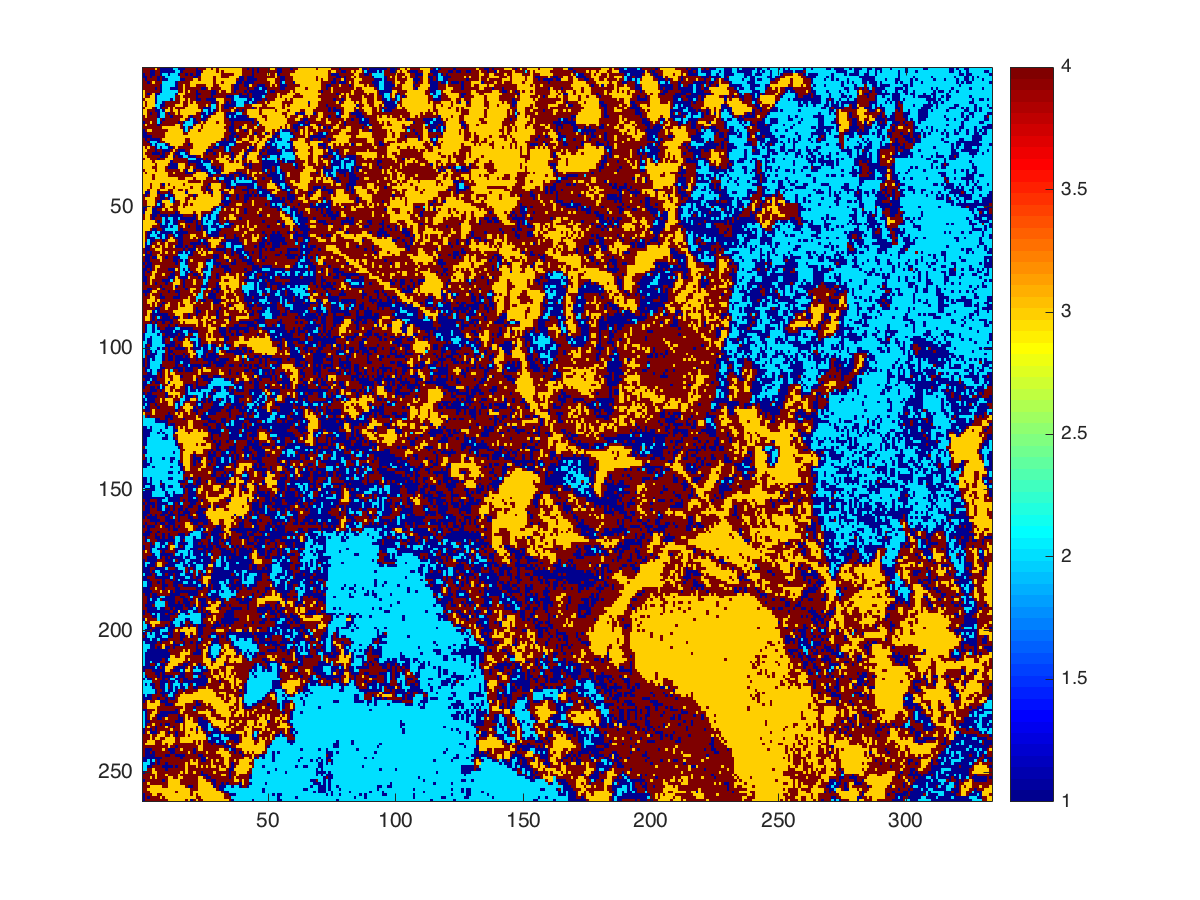
\includegraphics[width=1.0\textwidth]{Feature1ClassificationResult}	
	\caption*{Image 1}
	\end{subfigure}
	\begin{subfigure}{0.5\textwidth}
	\centering
	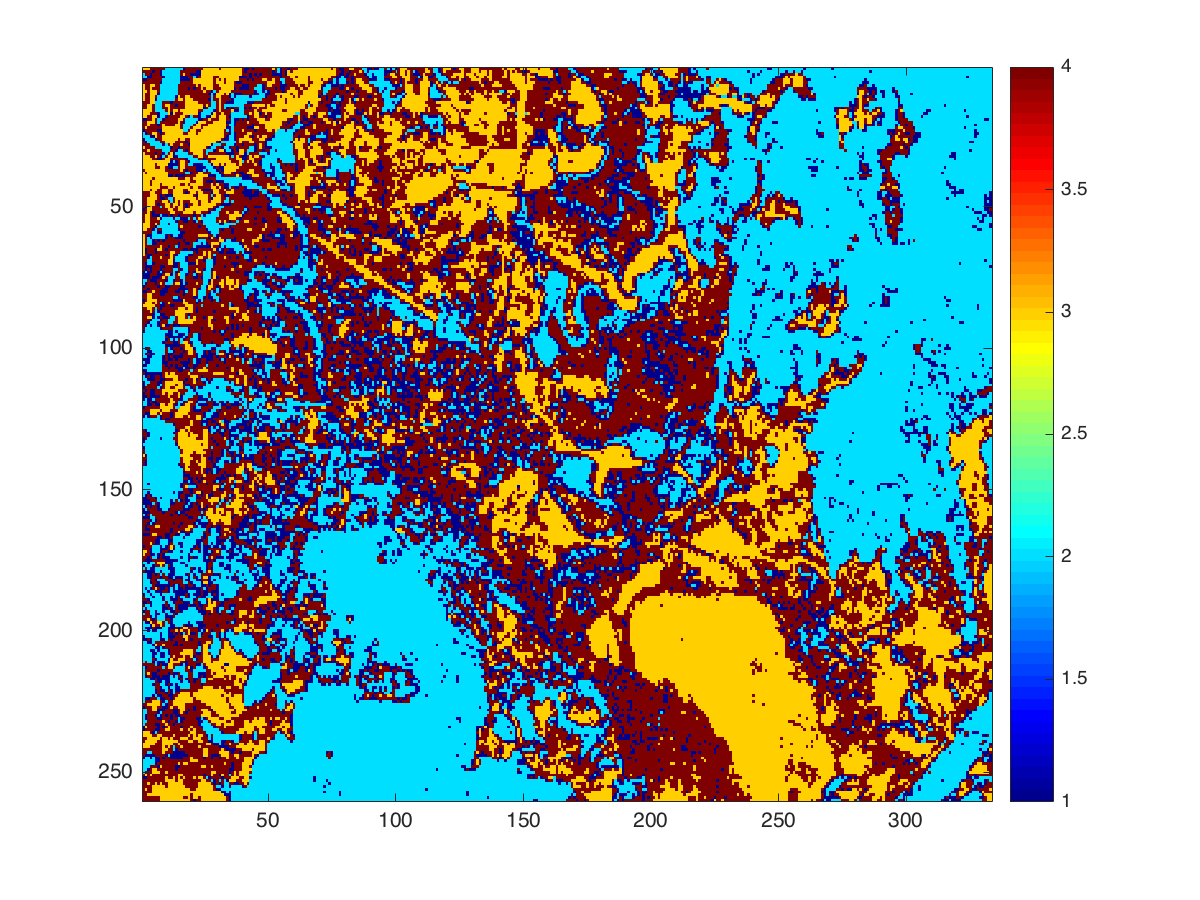
\includegraphics[width=1.0\textwidth]{Feature2ClassificationResult}
	\caption*{Image 2}
	\end{subfigure}
\end{figure}
\begin{figure}[!ht]
	\begin{subfigure}{0.5\textwidth}
	\centering
	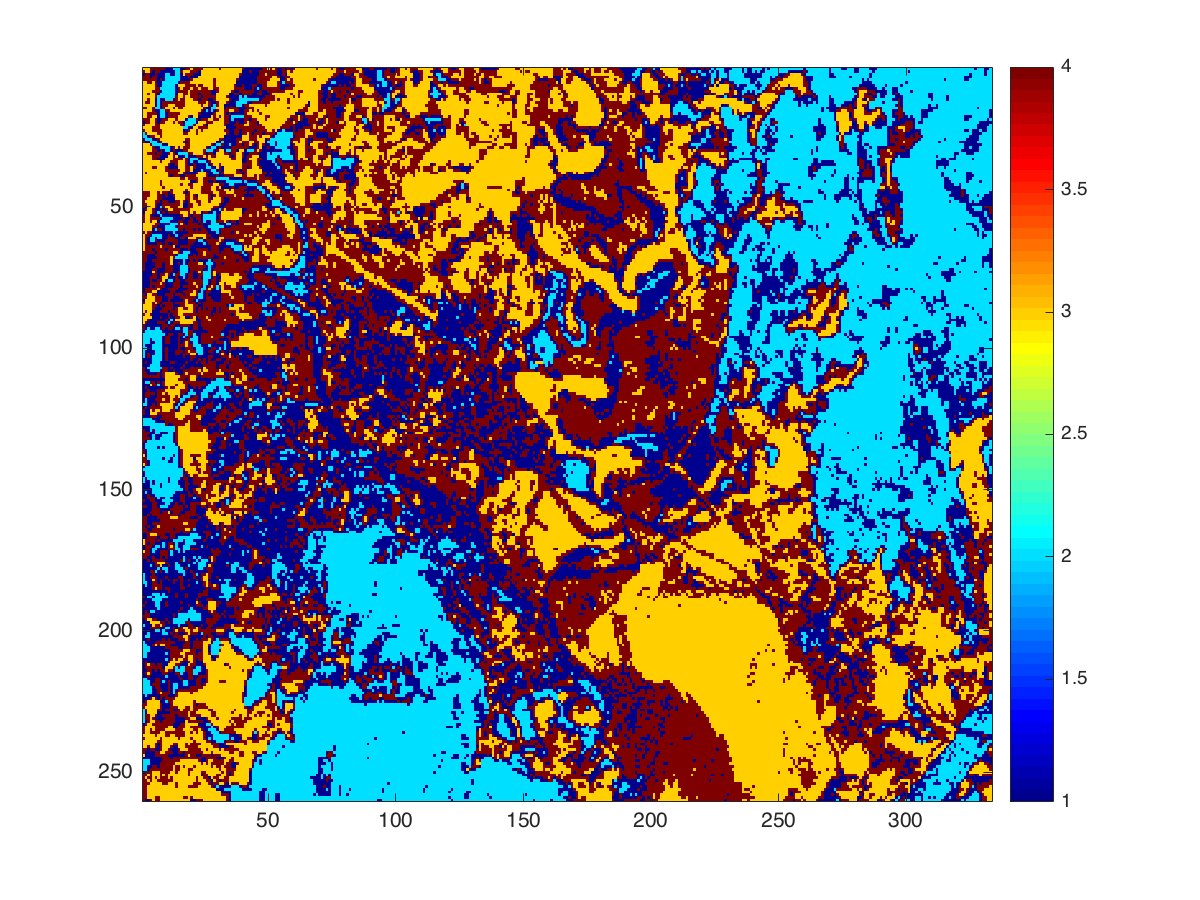
\includegraphics[width=1.0\textwidth]{Feature3ClassificationResult}	
	\caption*{Image 3}
	\end{subfigure} 
	\begin{subfigure}{0.5\textwidth}
	\centering
	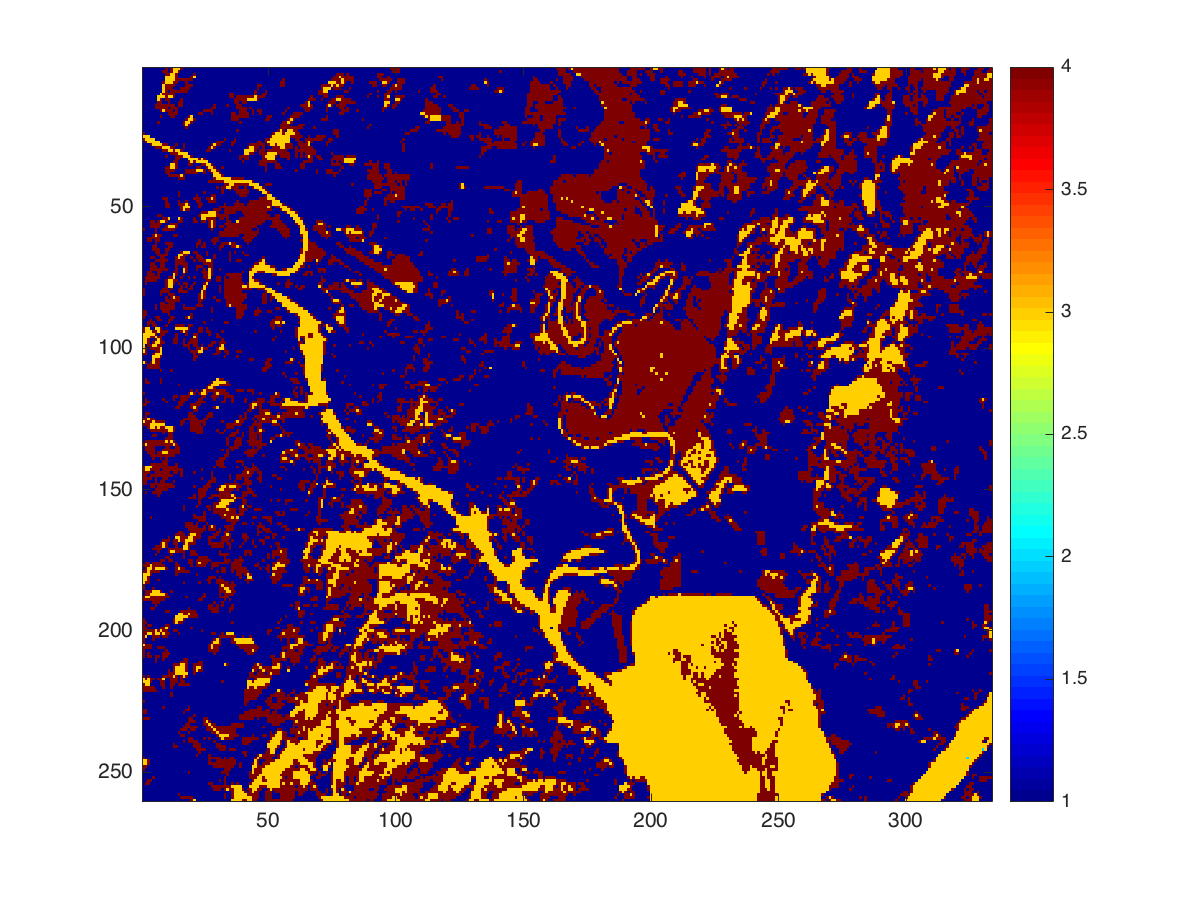
\includegraphics[width=1.0\textwidth]{Feature4ClassificationResult}	
	\caption*{Image 4}
	\end{subfigure}
\end{figure}
\begin{figure}[!ht]
	\begin{subfigure}{0.5\textwidth}
	\centering
	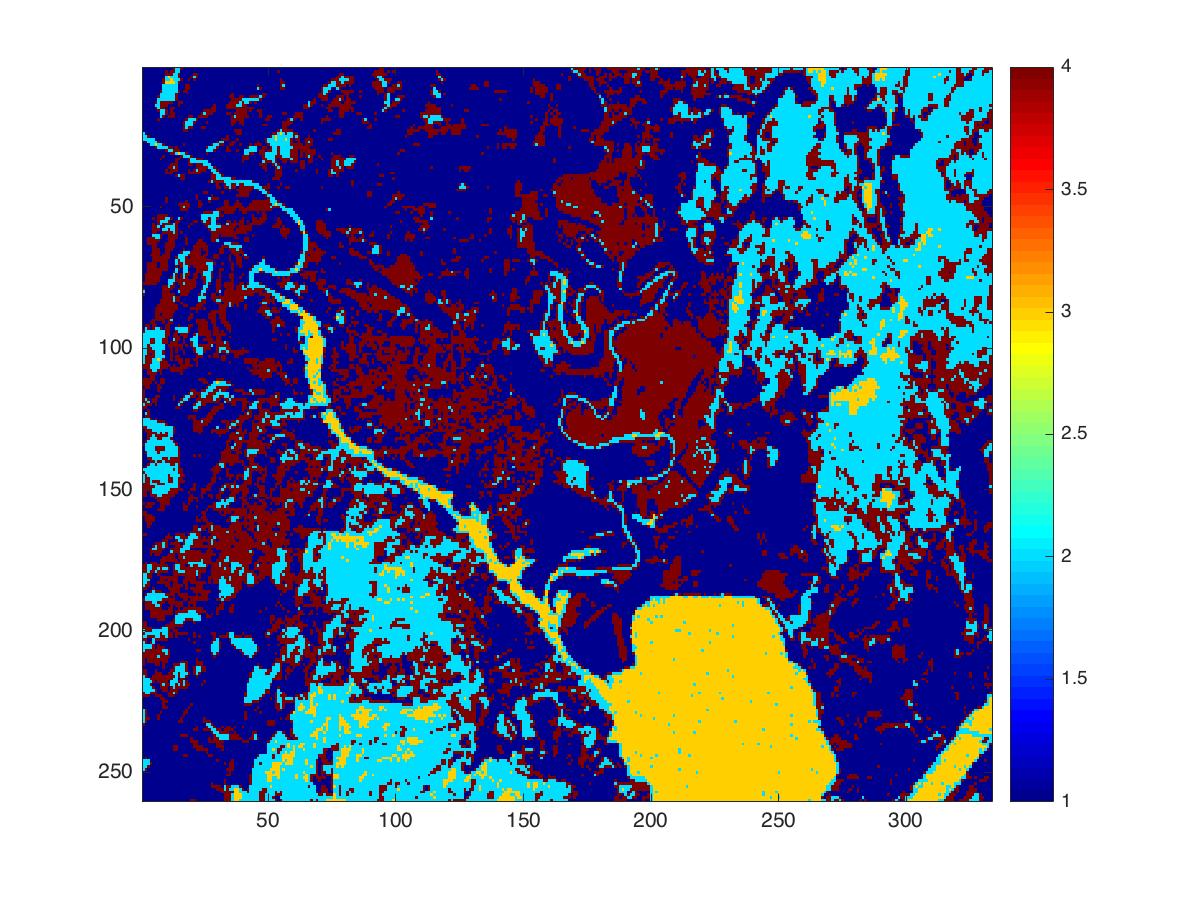
\includegraphics[width=1.0\textwidth]{Feature5ClassificationResult}	
	\caption*{Image 5}
	\end{subfigure}
	\begin{subfigure}{0.5\textwidth}
	\centering
	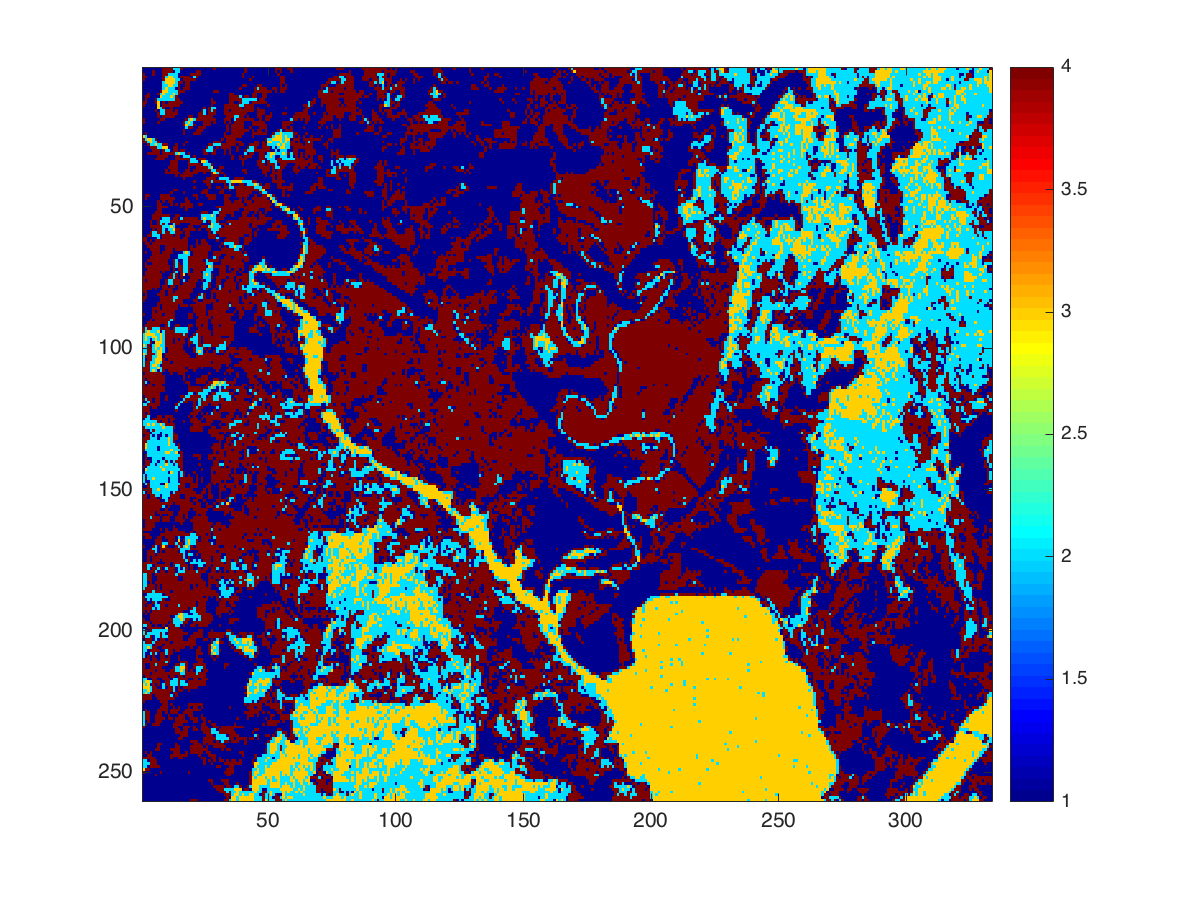
\includegraphics[width=1.0\textwidth]{Feature6ClassificationResult}	
	\caption*{Image 6}
	\end{subfigure}
	\caption{Classification results for each image}
\end{figure}

\section*{Testing and measuring error/success }

\section*{Conclusions}
As you can see this is a very simple way of classifying pixels and fails to take advantage of our 6 images and the mask to build a better statistical model for classification. However, it is still pretty cool that it works at all.

\end{document}